前章のように,日本では医療情報が全ての医療機関では共有されていない.
そこで,
患者が自身の医療情報を操作できて,
異なるフォーマットからの入力に
対応した医療情報を共有するシステムを提案する.
提案システムの設計を図\ref{system_construct},
図\ref{class}の
UMLユースケース図とUMLクラス図によって示す.

\begin{figure}[htbp]
  \begin{center}
    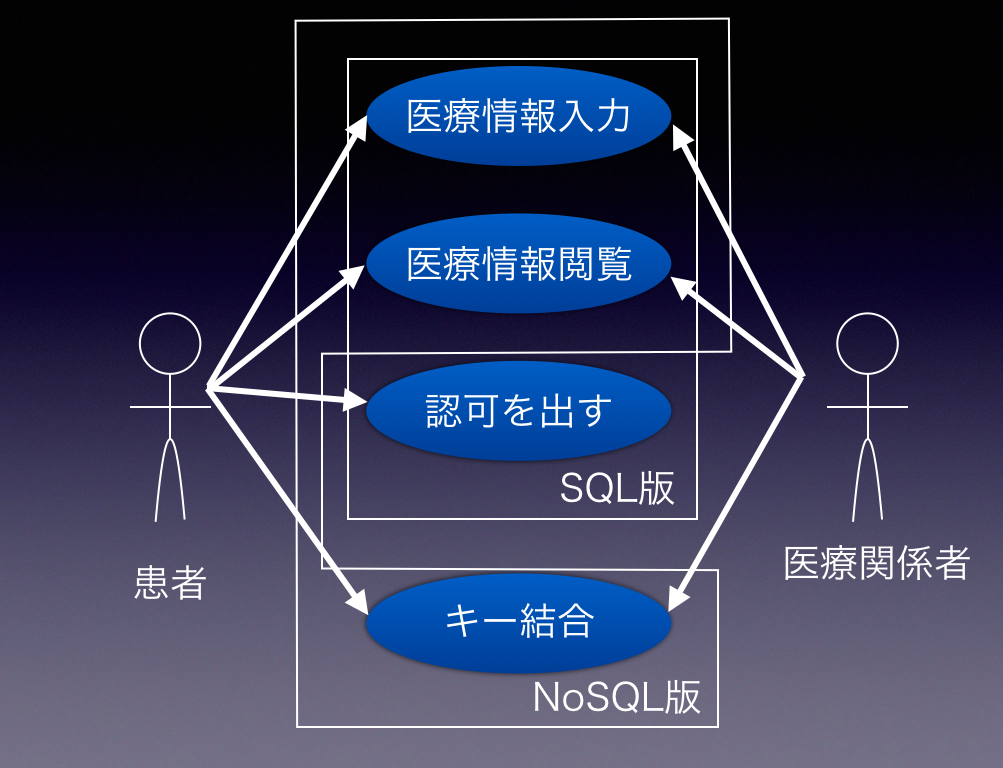
\includegraphics[width=10cm, bb=0 0 1003 768]{./gazou/system_construct2.png}
  \end{center}
  \caption{システムのUMLユースケース図}
  \label{system_construct}
\end{figure}

\begin{figure}[htbp]
  \begin{center}
    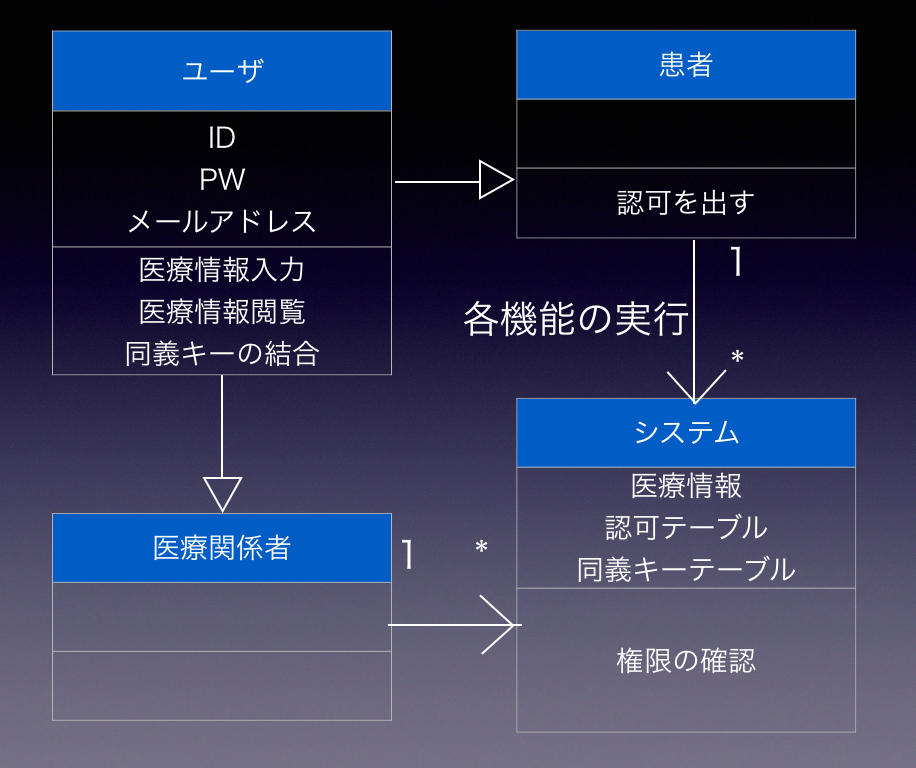
\includegraphics[width=10cm, bb=0 0 916 760]{./gazou/class.png}
  \end{center}
  \caption{UMLクラス図}
  \label{class}
\end{figure}

医療情報の入力と閲覧は既存のシステムにも導入されていて,
医療情報共有システムとして必須と言える.
%SQLデータベースを用いたシステムは医療情報を整形することができたので
%表とガントチャートによって医療情報を出力している.

認可を出す機能は患者が利用できる機能で,
自身の医療情報を操作できる医療関係者を選択するためのものである.

キー結合とはCouchDBを用いたシステムのための機能である.
異なる形式の入力データは同じ意味の項目であっても,
厳密に同じ言葉を項目名にとっていないことがある.
例えば薬を処方した日という意味の項目に対して処方日という項目名と
日時という項目名をとっている場合がある.
CouchDBからデータを抽出する際,これらを同義として抽出できなければ,
データがあるにもかかわらず,診断や処方の際に利用できない.

ここでは便宜的に処方日と日時のように,
異なる項目名であるが同じ意味の項目の群を
同義キーと呼ぶ.
この同義キーを関連付ける機能を実装することで
異なる形式からの入力情報を関連付ける.
具体的な機能として,同義キーのうちのひとつが検索される際に,
その同義キーの群の項目も検索結果として反映させる.
